\documentclass[dvipdfmx,cjk,xcolor=dvipsnames,envcountsect,notheorems,12pt]{beamer}
% * 16:9 のスライドを作るときは、aspectratio=169 を documentclass のオプションに追加する
% * 印刷用の配布資料を作るときは handout を documentclass のオプションに追加する
%   (overlay が全て一つのスライドに出力される)

\usepackage{pxjahyper}% しおりの文字化け対策 (なくても良い)
\usepackage{amsmath,amssymb,amsfonts,amsthm,ascmac,cases,bm,pifont}
\usepackage{graphicx}
\usepackage{url}

% スライドのテーマ
\usetheme{sumiilab}
% ベースになる色を指定できる
%\usecolortheme[named=Magenta]{structure}
% 数式の文字が細くて見難い時は serif の代わりに bold にしましょう
%\mathversion{bold}

%% ===============================================
%% スライドの表紙および PDF に表示される情報
%% ===============================================

%% 発表会の名前とか(省略可)
\session{ML勉強会}
%% スライドのタイトル
\title{信用できる言語\\Standard ML}
%% 必要ならば、サブタイトルも
%\subtitle{}
%% 発表者のお名前
\author{@fetburner}
%% 発表者の所属([] 内は短い名前)
%\institute[東北大学 住井・松田研]{東北大学 工学部 電気情報物理工学科\\住井・松田研究室}% 学部生
%\institute[東北大学 住井・松田研]{東北大学 大学院 情報科学研究科\\住井・松田研究室}% 院生
%% 発表する日
\date{2016年7月9日}

%% ===============================================
%% 自動挿入される目次ページの設定(削除しても可)
%% ===============================================

%% section の先頭に自動挿入される目次ページ(削除すると、表示されなくなる)
%% \AtBeginSection[]{
%% \begin{frame}
%%   \frametitle{アウトライン}
%%   \tableofcontents[sectionstyle=show/shaded,subsectionstyle=show/show/hide]
%% \end{frame}}
%% subsection の先頭に自動挿入される目次ページ(削除すると、表示されなくなる)
%% \AtBeginSubsection[]{
%% \begin{frame}
%%   \frametitle{アウトライン}
%%   \tableofcontents[sectionstyle=show/shaded,subsectionstyle=show/shaded/hide]
%% \end{frame}}

%% 現在の section 以外を非表示にする場合は以下のようにする

%% \AtBeginSection[]{
%% \begin{frame}
%%   \frametitle{アウトライン}
%%   \tableofcontents[sectionstyle=show/hide,subsectionstyle=show/show/hide]
%% \end{frame}}
%% \AtBeginSubsection[]{
%% \begin{frame}
%%   \frametitle{アウトライン}
%%   \tableofcontents[sectionstyle=show/hide,subsectionstyle=show/shaded/hide]
%% \end{frame}}

%% ===============================================
%% 定理環境の設定
%% ===============================================

\setbeamertemplate{theorems}[numbered]% 定理環境に番号を付ける
\theoremstyle{definition}
\newtheorem{definition}{定義}
\newtheorem{axiom}{公理}
\newtheorem{theorem}{定理}
\newtheorem{lemma}{補題}
\newtheorem{corollary}{系}
\newtheorem{proposition}{命題}

%% ===============================================
%% ソースコードの設定
%% ===============================================

\usepackage{listings,jlisting}
%\usepackage[scale=0.9]{DejaVuSansMono}

\definecolor{DarkGreen}{rgb}{0,0.5,0}
% プログラミング言語と表示するフォント等の設定
\lstset{
  language={[Objective]Caml},% プログラミング言語
  basicstyle={\ttfamily\small},% ソースコードのテキストのスタイル
  keywordstyle={\bfseries},% 予約語等のキーワードのスタイル
  commentstyle={},% コメントのスタイル
  stringstyle={},% 文字列のスタイル
  frame=trlb,% ソースコードの枠線の設定 (none だと非表示)
  numbers=none,% 行番号の表示 (left だと左に表示)
  numberstyle={},% 行番号のスタイル
  xleftmargin=5pt,% 左余白
  xrightmargin=5pt,% 右余白
  keepspaces=true,% 空白を表示する
  mathescape,% $ で囲った部分を数式として表示する ($ がソースコード中で使えなくなるので注意)
  % 手動強調表示の設定
  moredelim=[is][\itshape]{@/}{/@},
  moredelim=[is][\color{red}]{@r\{}{\}@},
  moredelim=[is][\color{blue}]{@b\{}{\}@},
  moredelim=[is][\color{DarkGreen}]{@g\{}{\}@},
}

%% ===============================================
%% 本文
%% ===============================================
\begin{document}
\frame[plain]{\titlepage}% タイトルページ

%% \section*{アウトライン}

% 目次を表示させる(section を表示し、subsection は隠す)
%% \begin{frame}
%%   \frametitle{アウトライン}
%%   \tableofcontents[sectionstyle=show,subsectionstyle=hide]
%% \end{frame}

\section{自己紹介}
\begin{frame}
	\frametitle{自己紹介}
	\begin{columns}
		\begin{column}{0.6\textwidth}
			\begin{itemize}
				\item ろんだ(@fetburner)
				\item 青葉山に篭ってCoqを書くM1
				\item MLが好き
			\end{itemize}
		\end{column}
		\begin{column}{0.3\textwidth}
			\begin{center}
				
\includegraphics[width=30mm]{icon.jpg}
			\end{center}
		\end{column}
	\end{columns}
\end{frame}

\section{アウトライン}

\begin{frame}
	\frametitle{今日の発表内容}
	\Large
	処理系の形式的検証についてのサーベイ

	\vfill

	CakeMLの紹介
\end{frame}

\section{背景}

\begin{frame}
	\frametitle{動機}
	\Large
	バグの無いプログラムが書きたい

	\vfill

	$\Rightarrow$テストを書こう!
\end{frame}

\begin{frame}
	\frametitle{テスト}
	\Large
	"Program testing can be used to show the presence of bugs, but never to show their absence!"
	(E.W. Dijkstra)

	\vfill

	テストだけでは力不足$\cdots$

	\vfill

	$\Rightarrow$形式手法の出番
\end{frame}

\begin{frame}
	\frametitle{形式手法}
	\Large
	プログラムの仕様を形式的に書き下して証明

	\vfill

	プログラムにバグがない事が数学的に保障
\end{frame}

\begin{frame}
	\frametitle{現実}
	\Large 
	プログラムの正しさは処理系の正しさに依存

	\vfill

	証明付きのプログラムも間違ったコンパイラでコンパイルしては正しく動かない$\cdots$

	\vfill

	$\Rightarrow$処理系も検証しよう!
\end{frame}

\section{関連研究}

\begin{frame}
	\frametitle{先行研究}
	\Large
	CompCert[Leroyら 2006]
	\begin{itemize}
		\item 言語処理系検証のマイルストーン
		\item 実用的なCコンパイラの検証
			\begin{itemize}
				\item ANSI Cの大部分をサポート
				\item PowerPC、ARM、x86のネイティブコードを出力
				\item GCCに匹敵するパフォーマンス
			\end{itemize}
		\item 大部分をCoqで検証
	\end{itemize}

	\vfill

	でもC言語なんて書きたくないよね$\cdots$
\end{frame}

\begin{frame}
	\frametitle{関数型言語の検証}
	\Large
	ML処理系を検証する試みも多数存在

	\begin{itemize}
		\item LambdaTamer[Clipala 2010]
		\item Pilsner[Neisら 2015]
		\item CakeML[Kumarら 2014]
	\end{itemize}

	\vfill

	今回は特にCakeMLに注目
\end{frame}

\section{CakeML}
\begin{frame}
	\frametitle{CakeML}
	\Large
	実用的なStandard ML処理系の検証
	\begin{itemize}
		\item ブートストラップにも成功
		\item ARMv6、ARMv8、MIPS-64、RISC-Vのネイティブコードを出力
		\item Poly/MLの数倍速い
	\end{itemize}

	HOL4による執拗なまでの証明
\end{frame}

\subsection{対象言語}

\begin{frame}
	\frametitle{対象言語}
	\Large
	Standard MLのサブセット
	\begin{itemize}
		\item 高階関数
		\item 副作用
			\begin{itemize}
				\item 参照
				\item 例外
			\end{itemize}
		\item ヴァリアント
		\item パターンマッチ
		\item モジュール
		\item 入出力
	\end{itemize}
\end{frame}

\begin{frame}
	\frametitle{対象言語の文法}
	\begin{center}
		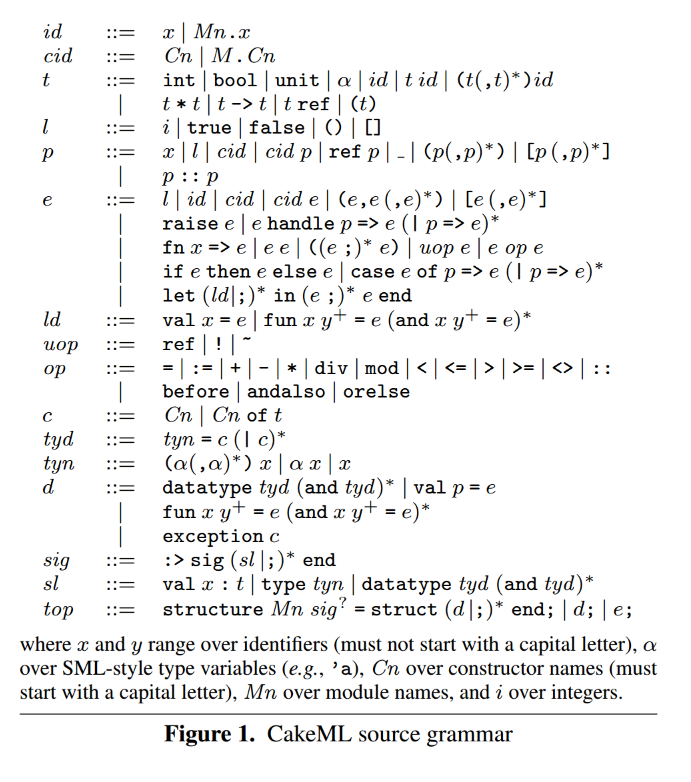
\includegraphics[width=80mm]{./syntax.png}
	\end{center}
\end{frame}

\begin{frame}[fragile]
	\frametitle{なぜStandard MLか?}
	\Large
	厳密な言語仕様
	\begin{columns}
		\begin{column}{0.55\textwidth}
			OCaml
			
			\vfill

\begin{lstlisting}
(print_string"Mt. ";1)
+(print_string"Aoba";2)
\end{lstlisting}

			\vfill

			未定義動作
		\end{column}
		\begin{column}{0.4\textwidth}
			Standard ML

			\vfill

\begin{lstlisting}
(print"Mt. ";1)
+(print"Aoba";2)
\end{lstlisting}

			\vfill

			"Mt. Aoba"と表示
		\end{column}
	\end{columns}
\end{frame}

\section{検証}

\begin{frame}
	\frametitle{検証の流れ}
	\Large
	REPLが使用を満たす事を証明してextract$\rightarrow$ブートストラップ

	今はx86バックエンドも証明済

	\begin{center}
		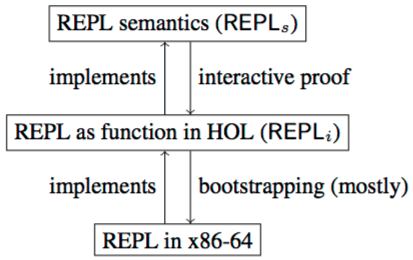
\includegraphics[width=80mm]{./verification.png}
	\end{center}
\end{frame}

\begin{frame}
	\frametitle{CakeMLの構成}
	\Large
	\begin{center}
		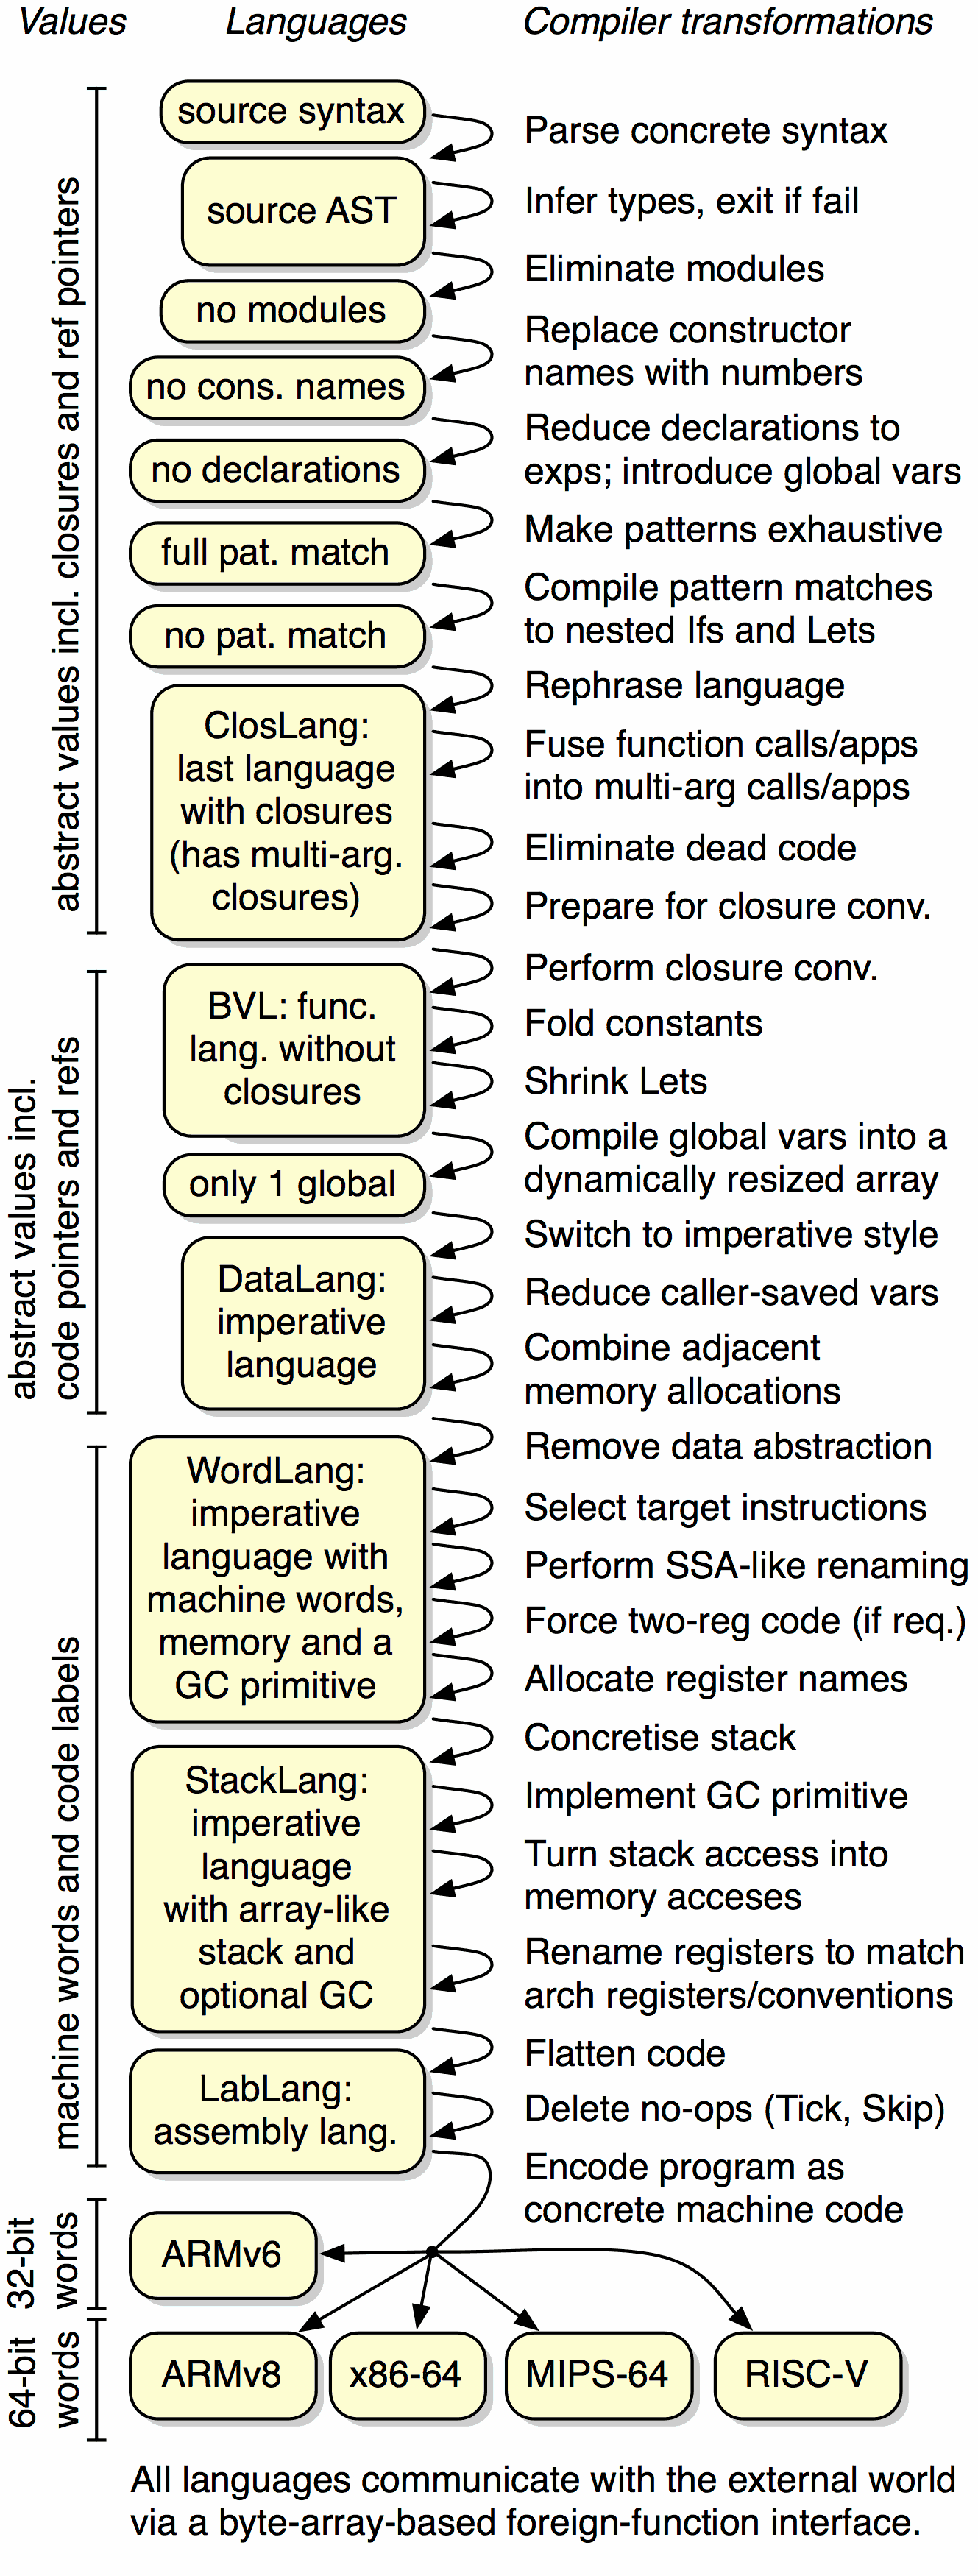
\includegraphics[width=25mm]{./phase.png}
	\end{center}
	コンパイルフェーズごとに証明して結合
\end{frame}

\begin{frame}
	\frametitle{パーサー}
	{\Large PEGで実装}
  \begin{theorem}[パーサーの健全性]
		PEGが非終端記号Nのパースに成功した場合、そのパース結果は文脈自由文法でのNの導出木と対応するトークンの列となる
  \end{theorem}
  \begin{theorem}[パーサーの完全性]
		入力に対応する構文解析木が存在する場合、PEGは構文解析に成功する
  \end{theorem}
\end{frame}

\begin{frame}
	\frametitle{型推論器}
	{\Large ML多相の型推論}
  \begin{theorem}[型推論の健全性]
		与えられたプログラムの型推論に成功した場合、そのプログラムには型を付けられる
  \end{theorem}
  \begin{theorem}[型推論の完全性]
		型を付けられるプログラムの型推論は成功する
  \end{theorem}
\end{frame}

\begin{frame}
	\frametitle{コード生成、最適化}
	\Large 入力されたプログラムと出力されたプログラムが等価であると期待

	\vfill

	変換前のプログラムの評価結果と変換後のプログラムの評価結果が対応している事を示す
\end{frame}

\begin{frame}
	\frametitle{結論}
	\large
	\only<1>{SMLにはこんなにも検証された処理系がある$\cdots$}

	\pause

	\Huge
	\only<2>{Standard MLは信用できる!}
\end{frame}

\end{document}
